% !TEX root= ../main.tex
\section{Discourse Theories and Digraphs}
\label{sec:Discourse Theories and Digraphs}
As mentioned earlier, there is a close connection between (1) models of a discourse, (2) kernels in a graph and (3) solutions of a graph.
While we have the equivalence between (2) and (3), we will now look at two functions connecting (1) and (2).
This correspondence was shown by Roy T. Cook in \cite{cook}.
We get the following definitions from \cite{apal-digraph}.

$\mathcal{T}:$ translating a digraph \textbf{G} into a corresponding theory $\mathcal{T}(\mathbf{G})$ such that $sol(\mathbf{G}) = mod(\mathcal{T}(G))$.

$\mathcal{G}:$ translating a theory $T$ into a corresponding digraph $\mathcal{G}(T)$ such that $mod(T) = sol(\mathcal{G}(T))$.

Given any digraph \textbf{G} we get the theory $\mathcal{T}(\mathbf{G})$ by taking, for each $x \in G$, the formula $x \leftrightarrow \bigwedge_{y \in N(x)} \neg y$ where $\bigwedge \emptyset = 1$.\par
\begin{figure}[!h]
  \centering
  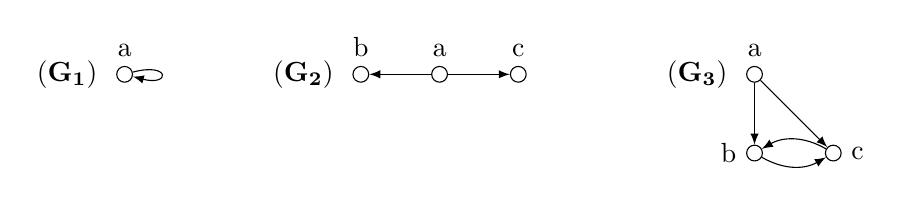
\begin{tikzpicture}
    [
    point/.style={circle,draw,inner sep=0pt,minimum size=2mm},
    collection/.style={thick,rectangle,draw,inner sep=0pt,minimum height=14mm, minimum width= 9mm}
    ]
    \node (label) at (0,1) [label=left:$(\mathbf{G_1})\;$] {};
    \node (0) at (0,1) [point,label=above:a] {};
    \draw [-latex, loop right] (0) to (0);

    \node (label) at (3,1) [label=left:$(\mathbf{G_2})\;$] {};
    \node (0) at (4,1) [point,label=above:a] {};
    \node (1) at (3,1) [point,label=above:b] {};
    \node (2) at (5,1) [point,label=above:c] {};
    \draw [-latex] (0) to (1);
    \draw [-latex] (0) to (2);

    \node (label) at (8,1) [label=left:$(\mathbf{G_3})\;$] {};
    \node (0) at (8,1) [point,label=above:a] {};
    \node (1) at (8,0) [point,label=left:b] {};
    \node (2) at (9,0) [point,label=right:c] {};
    \draw [-latex] (0) to (2);
    \draw [-latex] (0) to (1);
    \draw [-latex, bend right] (1) to (2);
    \draw [-latex, bend right] (2) to (1);
  \end{tikzpicture}
  \caption{}
  \label{ex:3graphs}
\end{figure}
  The graphs in Figure~\ref{ex:3graphs} have the following theories:
\begin{align}
  \mathcal{T}(\mathbf{G_1}) &= \big \{ a \leftrightarrow \neg a \big \} \\
  \mathcal{T}(\mathbf{G_2}) &= \big \{ a \leftrightarrow (\neg b \wedge \neg c), b, c \big \}\\
  \mathcal{T}(\mathbf{G_3}) &= \big \{ a \leftrightarrow (\neg b \wedge \neg c), b \leftrightarrow \neg c, c \leftrightarrow \neg b \big \}
\end{align}
The fact that $sol(\mathbf{G}) = mod(\mathcal{T}(G))$ is shown in \cite{apal-digraph}.
All though not proving it, we observe that $\mathbf{G_1}$ has no solution, just like its corresponding theory $\mathcal{T}(\mathbf{G_1})$ has no models.
$\mathbf{G_2}$ has one solution, where one assigns $a=0, b=1, c=1$.
This assignment also works as the only model for $\mathcal{T}(\mathbf{G_2})$.
In $\mathbf{G_3}$, we get two solutions, both with $a$ assigned 0, but with 0 and 1 distributed between $b$ and $c$.
These are also the only two models of $\mathcal{T}(\mathbf{G_3})$.

Conversely, given any discourse theory $T$ (in fact, this will work given any PL theory, since we can translate CNF to GNF), we can derive the corresponding graph $\mathcal{G}(T)$ in the following way:
All variables in the theory are vertices, and for each formula $x \leftrightarrow \bigwedge_{y \in I_x} y$ make a directed edge $\langle x,y \rangle$ for each $y \in I_x$.
  \begin{align}
    T = \{ ( a \lar \neg a'), (a' \lar \neg a), (b \lar \neg b'), (b' \lar \neg b), (y_1 \lar (\neg a \wedge \neg b \wedge \neg y_1)) \}
  \end{align}
  Using $\mathcal{G}$ on the above GNF theory gives us the following graph:\par
  \begin{figure}[!h]
    \centering
    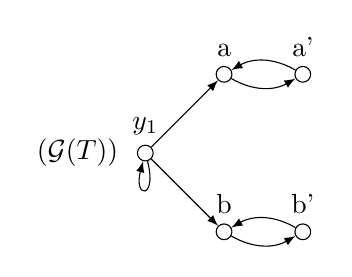
\begin{tikzpicture}
      [
      point/.style={circle,draw,inner sep=0pt,minimum size=2mm},
      collection/.style={thick,rectangle,draw,inner sep=0pt,minimum height=14mm, minimum width= 9mm}
      ]
      \node (label) at (5,1) [label=left:$(\mathcal{G}(T))\;$] {};
      \node (0) at (5,1) [point,label=above:$y_1$] {};
      \node (1) at (6,0) [point,label=above:b] {};
      \node (2) at (7,0) [point,label=above:b'] {};
      \node (3) at (6,2) [point,label=above:a] {};
      \node (4) at (7,2) [point,label=above:a'] {};
      \draw [-latex, loop below] (0) to (0);
      \draw [-latex] (0) to (1);
      \draw [-latex, bend right] (1) to (2);
      \draw [-latex, bend right] (2) to (1);
      \draw [-latex] (0) to (3);
      \draw [-latex, bend right] (3) to (4);
      \draw [-latex, bend right] (4) to (3);
    \end{tikzpicture}
    \caption{}
    \label{ex:graph_from_theory}
\end{figure}
Again, will we not be proving the correspondence, but notice that $T$ has three solutions, where either $a$, $b$ or both are assigned $1$.
This reflects onto the graph where $y_1$ has to be assigned $0$, thus forcing $a$ or $b$ to be assigned $1$.
The fact that $\mathcal{G}$ gives us the correspondence we are looking for is shown in \cite{apal-digraph}.

With the problem of solutions in the graph being equivalent with SAT, we get our final equivalence between kernels in the graph and models of the theory.
More precisely, we have that the set of kernels in a graph is equivalent with the set of models of the corresponding theory.
Because of this tight link, we might refer to graphs without kernels as paradoxical graphs.

The applicability of kernels should by now be obvious.
In the next section we will review various findings within Kernel Theory, and especially the findings related to infinitary graphs.
